% !TeX root = ../main.tex

\chapter{Benchmark}

\section{Benchmark Introduction}

We can benchmark a scheduler by many factors, for example, CPU utilization, throughput, turnaround time, latency, waiting time and etc. In this chapter, we will benchmark throughput, latency and turnaround time of SCHED\_NORMAL, SCHED\_FIFO, SCHED\_RR and SCHED\_RAS scheduling algorithms. 

\section{Benchmark Design}

First, we will explain the meaning of these test items in detail:
\begin{itemize}
    \item \textbf{throughput}: number of tasks that complete their execution per time unit.
    \item \textbf{latency}: time interval between the arrival of the task and the first execution of the task.
    \item \textbf{turnaround time}: time interval between the arrival of the task and the completion of the task.
\end{itemize}

We know that using Memory Access Tracing as the basis, RAS is write-sensitive. Thus, our benchmark program is I/O bound. The benchmark program will using \textit{mmap} system call to request a block of memory. We trace this memory's access using the tracer we implemented in Chapter One. Then benchmark program will fork a given number of child tasks to write random times into the memory. The four scheduling policies will be used in rotation under the same conditions.

\section{Benchmark Results}
\subsection{Throughput}

First, we benchmark the total running time of different scheduling policies with different task numbers. Each benchmark performs an average of 16368 writes per 10 tasks. The results are shown as following table:

\begin{table}[!hpt]
  \caption{Time Consumption of Each Benchmark (s)}
  \label{tab:firstone}
  \centering
  \begin{tabular}{*{6}{c}} \toprule
    \multirow{2}*{SCHED} & \multicolumn{5}{c}{Task Number} \\ \cmidrule(r){2-6}
    & 20 & 40 & 60 & 80 & 100 \\ 
    \midrule
    NORMAL & 22.259&30.568 &35.777 &41.616 & 50.145\\
    FIFO   & 7.441&15.152 &21.938 &28.863 & 37.169\\
    RR & 7.166&15.089 &21.776 &28.040 & 37.493\\
    RAS & 6.140&11.952 &17.358 &22.330 & 29.473\\
    \bottomrule
  \end{tabular}
\end{table}

It is apparent to see that RAS takes the least amount of time to complete the write tasks. FIFO and RR have nearly the same performance. NORMAL has the worst performance. Compared to FIFO and RR, RAS has about $20\%$ optimazation.

With the time consumption and task number of each scheduling algorithm, we can compute their throughput, number of tasks divided by time consumption. The results are as following chart:

\begin{figure}[!htp]
  \centering
  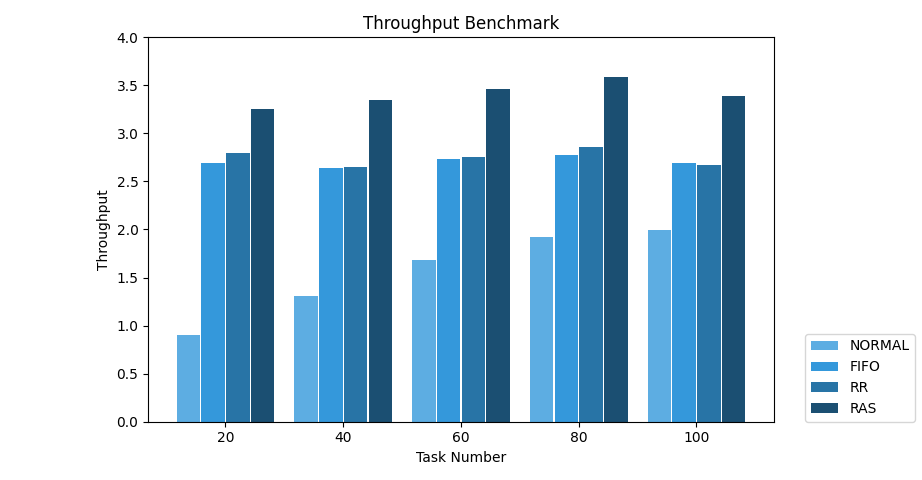
\includegraphics[width=13cm]{figures/throughput.png}
  \caption{Throughput Benchmark Result}
\end{figure}

In this chart we can see that RAS gets the highest throughput. For different task numbers, the throughput is about $3.4$ tasks per second. When the task number is too large, scheduling overhead may affect the throughput performance.

\subsection{Turnaround Time}

We record the fork time of a task and the completion time of it. And the turnaround time is their difference. A task will write minimum 16 times and maximum 8192 times. The results are as following chart:

\begin{figure}[!htp]
  \centering
  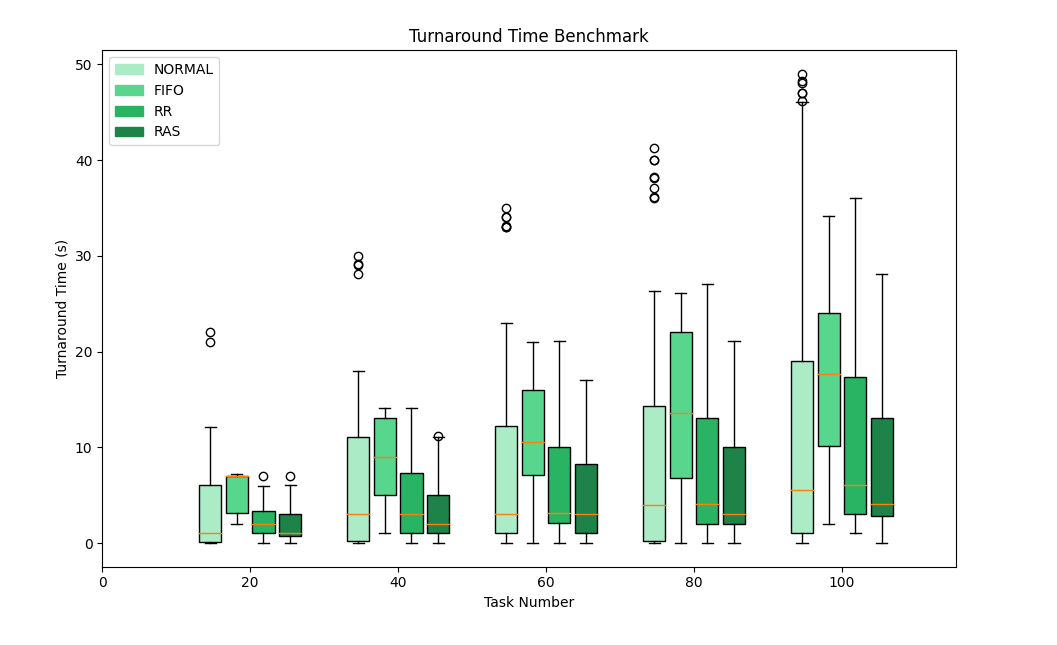
\includegraphics[width=13.5cm]{figures/turnaroundbox.png}
  \caption{Turnaround Time Benchmark Result}
  \label{fig:turnaroundbox}
\end{figure}

It is crystal clear that RAS gains the lowest average, the lowest median and the lowest upper boundary turnaround time. Besides, RAS also has the fewest outliers. It proves that among the four scheduler, RAS has the best and the most stable performance. Furthermore, we can notice that as the number of tasks increases, RAS will get better performance. And when task number is relatively low, RAS will achieve a similar performance to RR. This can be easily explained by the limited race situation when the number of tasks is small. Under these circumstances, the RAS will nearly allocate all the tasks with the maximum timeslice.

\subsection{Latency}

We use the difference between the fork time of a task and the first execution time to represent the latency. Also we choose 20, 40, 60, 80 and 100 task numbers and write minimum 16 times, maximum 8192 times. The results are as following chart:

\begin{figure}[!htp]
  \centering
  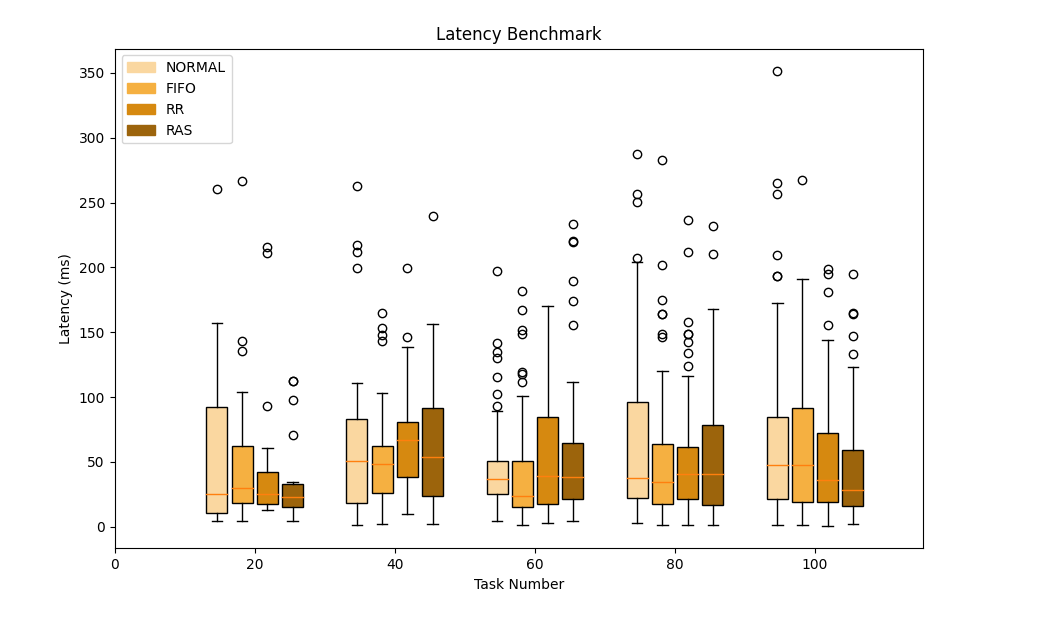
\includegraphics[width=13.5cm]{figures/latencybox.png}
  \caption{Latency Benchmark Result}
  \label{fig:turnaroundbox}
\end{figure}

In this chart we can find that RAS does not achieve great advantage in latency. The performances of RAS and RR are almost the same. The reason is that to reduce the overhead of context switch, we set the maximum timeslice (100ms, the same as RR timeslice) as the initial timeslice to RAS tasks. Therefore, when tasks first enter the kernel, they will be allocated with 100ms timeslice to run. That results in a larger latency for other tasks waiting for CPU. But compared to NORMAL and FIFO policies, RAS still gains optimization.


